\documentclass[a4paper,10pt]{article}

% Packages
\usepackage{graphicx}
\usepackage{amsmath}
\usepackage{geometry}
\usepackage{fancyhdr}
\usepackage{setspace}
\usepackage{float}
\usepackage{titlesec}  % For title formatting
\geometry{margin=1in}
\usepackage{caption}
\usepackage{subcaption}
\usepackage{booktabs}
\usepackage{multicol}
\usepackage{wrapfig}
\geometry{left=0.8in, right=0.8in, top=1.2in, bottom=1.2in}
\setstretch{0.95}

% Header and Footer
\pagestyle{fancy}
\fancyhf{}
\fancyhead[L]{Challenge 1}
\fancyhead[R]{\thepage}

% Title Formatting
\titleformat{\section}{\normalfont\Large\bfseries}{\thesection}{1em}{}

% Cover Page
\title{
    \vspace{2cm} % Adjust vertical space
    
\includegraphics[width=0.55\textwidth]{Logo_Polimi.png} \\ % Add your logo here (change "logo.png" to the actual filename)
    \vspace{1cm} % Adjust vertical space after the logo
    \textbf{\Huge Challenge 2} \\
    \vspace{1cm} % Adjust vertical space
    \large Advanced Algorithms and Parallel Programming \\
    \vspace{0.5cm} % Adjust vertical space
    \large \date{\today}
}

\author{Camilo José Sinning López, Oliver Mosgaard Stege\\ \& Raul Eduardo Vergara Lacouture}


\begin{document}

% Title Page
\maketitle
\thispagestyle{empty}
\newpage

% Table of Contents
% Start page numbering from the Table of Contents
\setcounter{page}{1}  % Start counting from 1
% \tableofcontents
% \newpage

\begin{multicols}{2} 
\section{Experimental Setup}

The program implements a parallel Sudoku solver using OpenMP. The algorithm recursively explores all possible solutions to a given Sudoku puzzle by assigning numbers to unfilled cells, ensuring no conflicts in rows, columns, or subgrids.

\subsection{Hardware and software}

All experiments were conducted on a laptop with the following processor details:

\begin{itemize}
    \item \textbf{Model:} AMD Ryzen 5 7520U with Radeon Graphics
    \item \textbf{Base Clock:} 2.8 GHz
    \item \textbf{Max Boost Clock:} Up to 4.3 GHz
    \item \textbf{Cores:} 4
    \item \textbf{Threads:} 8
\end{itemize}

Since the processor has 8 threads, but the experiments were conducted with thread counts ranging from 1 to 12, the results also include the execution time for thread counts higher than the number of available threads to assess the impact of the overhead of creating additional threads.

\subsection{Algorithm parameters}

\begin{itemize}
    \item Grid Size: Dimension of the Sudoku puzzle (e.g., 9x9).
    \item Block Size: Size of subgrids (e.g., 3x3 for standard Sudoku).
    \item Max Depth: Specifies the depth for task creation in the parallel recursion.
    \item Threads: Maximum number of threads to use in the parallel algorithm.
    \item sudoku: The Sudoku puzzle to solve.
\end{itemize}

\subsection{Executions}

\subsubsection{Fixed depth}

The first set of experiments was conducted with a fixed max\_depth of 3. For each thread count, 3 samples were collected for 9x9 and 16x16 Sudoku puzzles. On the other hand, the 25x25 Sudoku puzzle was only tested once per thread count due to the high execution time.

\subsubsection{Variable depth}
The second set of experiments was conducted with a variable max\_depth. For thread counts ranging from 1 to 12, experiments were conducted for each max\_depth value in {3, 5, 7, 9}. Three samples were collected for each 9x9 and 16x16 Sudoku.


% \section{Performance Measurements}

% Summarized results are saved in a CSV file with columns:

% \begin{enumerate}
%     \item Execution time.
%     \item Grid size.
%     \item Block size.
%     \item Number of threads.
%     \item Number of solutions.
%     \item Max depth.
% \end{enumerate}

% Sample output: The program outputs the timing and results to the console and appends them to the times.csv file.

\section{Results}

The following results were taken from times.csv file, and only the threads available in the machine were used for to create the plots since more threads would not be beneficial.

\subsection{Fixed depth}

In the fixed-depth experiments, the results indicate that overall increasing the number of threads lead to performance improvements in the parallel Sudoku solver. The 16x16 Sudoku puzzles (Figure~\ref{fig:16x16_fixed_depth}) show consistent reductions in execution time as the number of threads increases. The 25x25 Sudoku puzzle (Figure~\ref{fig:25x25_fixed_depth}) also demonstrates similar trends, although in 4 threads the execution time is higher than in 2 threads. The 9x9 Sudoku puzzles (Figure~\ref{fig:9x9_fixed_depth}) exhibit more variability, with some thread configurations performing worse than others. These results suggest that the performance gains from parallelization are more pronounced in larger Sudoku puzzles, where the overhead of task creation is amortized over more work.

\begin{figure}[H]
    \centering
    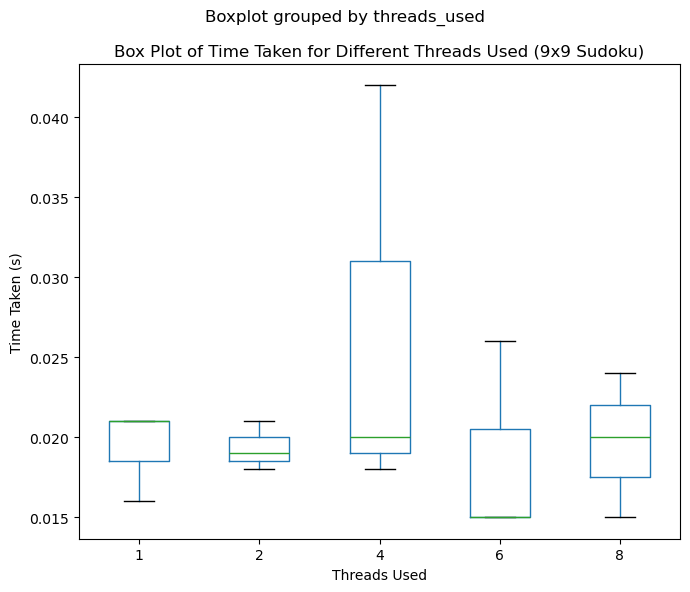
\includegraphics[width=0.3\textwidth]{9x9_fixed_depth.png}
    \caption{Execution time for 9x9 Sudoku puzzles with fixed depth.}
    \label{fig:9x9_fixed_depth}
\end{figure}

\begin{figure}[H]
    % \vspace{-0.5cm}
    \centering
    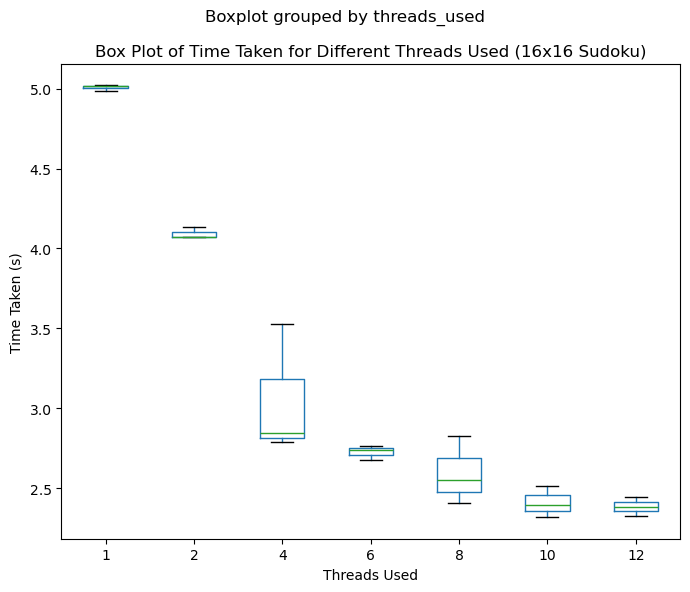
\includegraphics[width=0.3\textwidth]{16x16_fixed_depth.png}
    \caption{Execution time for 16x16 Sudoku puzzles with fixed depth.}
    \label{fig:16x16_fixed_depth}
\end{figure}

\begin{figure}[H]
    % \vspace{-1.5cm}
    \centering
    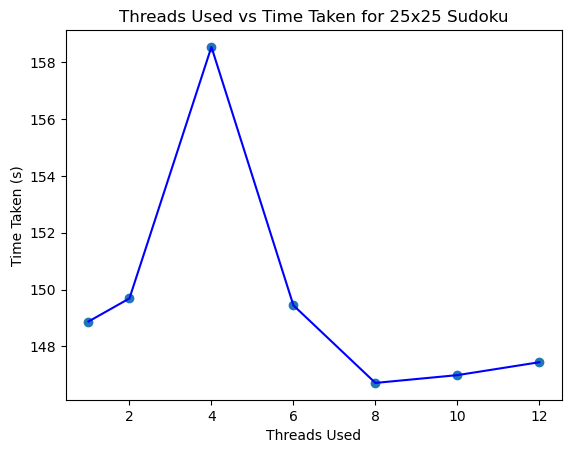
\includegraphics[width=0.3\textwidth]{25x25_fixed_depth.png}
    \caption{Execution time for 25x25 Sudoku puzzles with fixed depth.}
    \label{fig:25x25_fixed_depth}
\end{figure}

% \begin{figure}[H]
%     \caption{Comparison of execution times for fixed depth Sudoku puzzles.}
%     \centering
%     \begin{subfigure}[b]{0.3\textwidth}
%         \centering
%         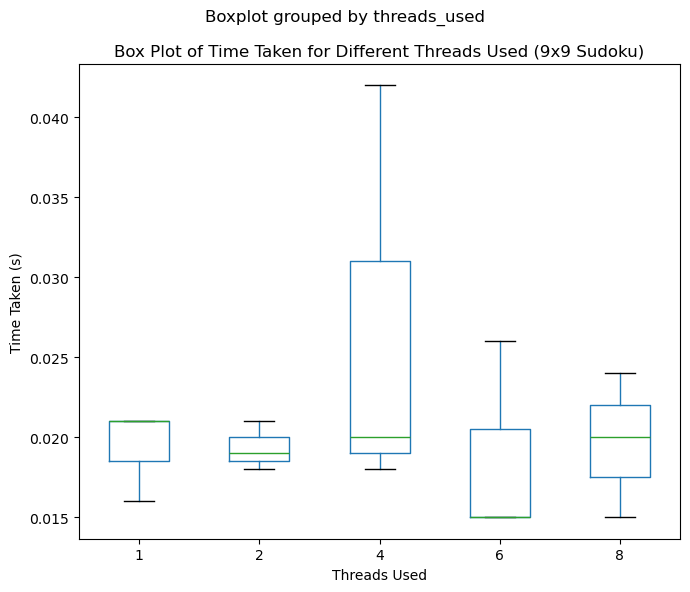
\includegraphics[width=\textwidth]{9x9_fixed_depth.png}
%         \caption{Execution time for 9x9 Sudoku puzzles with fixed depth.}
%     \end{subfigure}
%     \hfill
%     \begin{subfigure}[b]{0.3\textwidth}
%         \centering
%         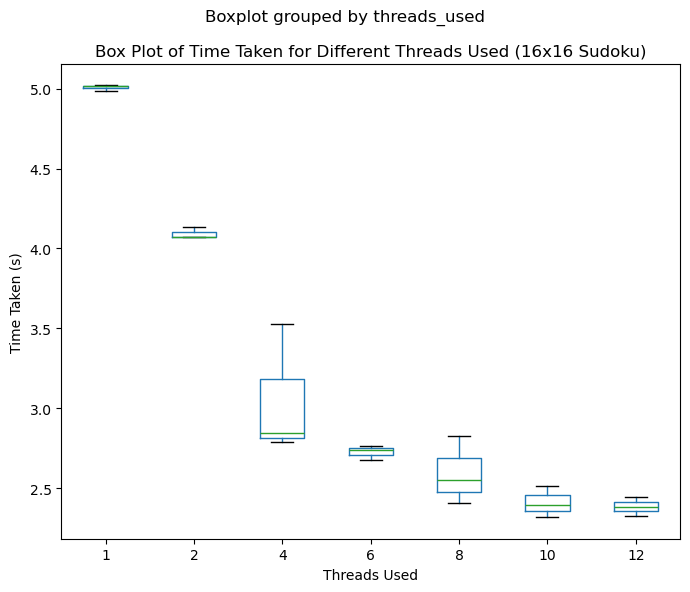
\includegraphics[width=\textwidth]{16x16_fixed_depth.png}
%         \caption{Execution time for 16x16 Sudoku puzzles with fixed depth.}
%     \end{subfigure}
%     \hfill
%     \begin{subfigure}[b]{0.3\textwidth}
%         \centering
%         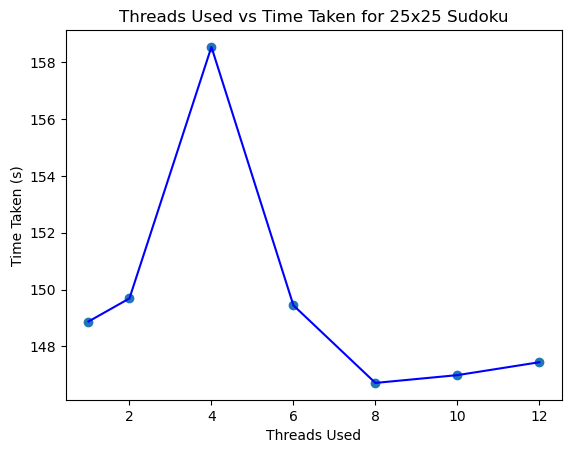
\includegraphics[width=\textwidth]{25x25_fixed_depth.png}
%         \caption{Execution time for 25x25 Sudoku puzzles with fixed depth.}
%     \end{subfigure}
% \end{figure}

\subsection{Variable depth}

\begin{figure}[H]
    % \vspace{-1.5cm}
    \centering
    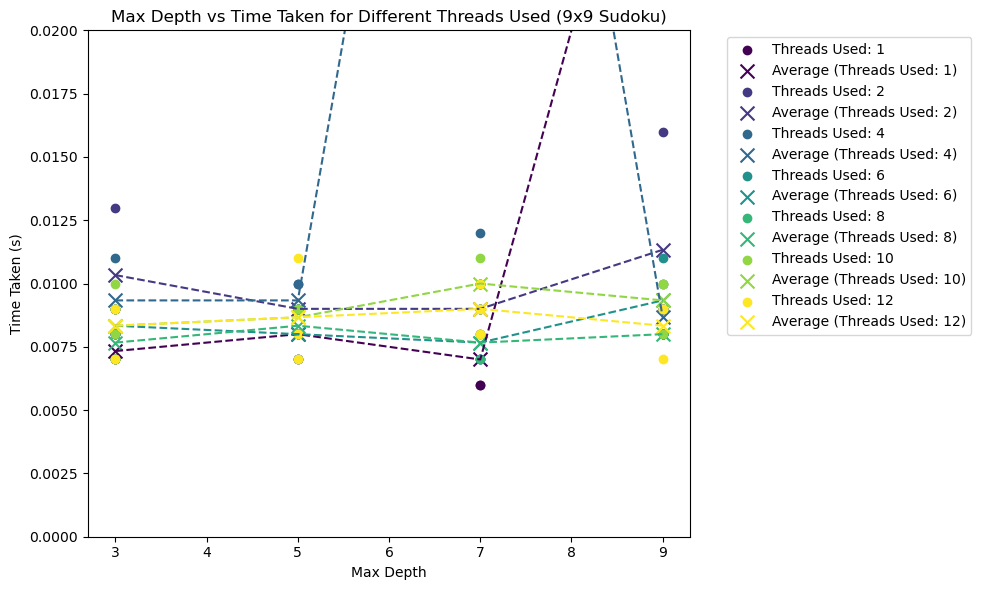
\includegraphics[width=0.4\textwidth]{9x9_var_depth.png}
    \caption{Execution time for 9x9 Sudoku puzzles with variable depth.}
    \label{fig:9x9_var_depth}
\end{figure}

\begin{figure}[H]
    \centering
    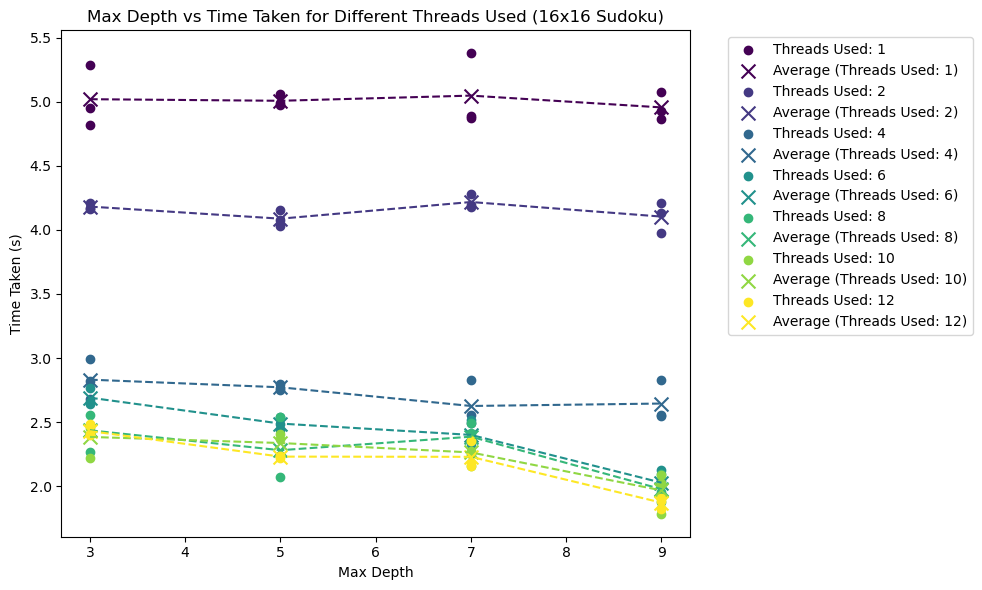
\includegraphics[width=0.4\textwidth]{16x16_var_depth.png}
    \caption{Execution time for 16x16 Sudoku puzzles with variable depth.}
    \label{fig:16x16_var_depth}
\end{figure}

For variable-depth experiments, performance trends are similarly unclear for the 9x9 Sudoku puzzle (Figure~\ref{fig:9x9_var_depth}), while the 16x16 Sudoku puzzle (Figure~\ref{fig:16x16_var_depth}) shows more consistent improvements with more threads. Although none of them seemed to have a clear trend with respect to the depth of the recursion.

\section{Design Choices}

\begin{enumerate}
    \item \textbf{Parallelization with OpenMP:} The algorithm uses OpenMP to parallelize the Sudoku solving process. More specifically using the tasks directive.
    \item \textbf{Recursive Backtracking:} The core of the algorithm is a recursive backtracking approach.
    \item \textbf{Depth Limitation:} To control the granularity of parallel tasks and avoid excessive task creation, the algorithm limits the depth of parallel recursion using the depth and max\_depth parameters.
    \item \textbf{Board Copying:} To avoid shared state issues between parallel tasks, the algorithm creates a copy of the Sudoku board for each task.
    \item \textbf{CSV Logging:} The algorithm logs the performance data to a CSV file.
\end{enumerate}

\section{Conclusions}

In summary, the parallel Sudoku solver demonstrates performance improvements with increasing thread counts, especially for larger Sudoku puzzles. The fixed-depth experiments show consistent reductions in execution time as the number of threads increases, while the variable-depth experiments exhibits small changes in performance. The results suggest that the parallel algorithm is effective in reducing the execution time of Sudoku puzzles, particularly for larger grid sizes.

\end{multicols}
\end{document}
